\documentclass[a4paper,12pt]{article}
\usepackage[T1]{fontenc}
\usepackage{lmodern}
\usepackage[english,spanish]{babel}
\usepackage[utf8]{inputenc}
\usepackage{hyperref}
\usepackage{fullpage}

\usepackage{graphicx}
\graphicspath{{./img/}}

\usepackage{csquotes}
\usepackage[
	backend=bibtex,
	bibencoding=ascii,
	style=numeric,
	sorting=none
]{biblatex}
\bibliography{ia-tp2}

\begin{document}

\section{Descripción del problema}

El problema que deseamos resolver es el problema de las $n$ reinas,
que es el caso general del problema de las ocho reinas.
Consiste en ubicar $n$ reinas en un tablero de ajedrez de $n \times n$ sin que se amenacen entre sí\cite{weisstein}.

La solución convencional a este problema fue propuesta por Dijkstra en 1972,
que utiliza búsqueda en profundidad con \foreignlanguage{english}{backtracking} para encontrar posibles posiciones para las $n$ reinas.
Sin embargo, este método no escala para valores de $n$ arbitrarios,
por lo que proponemos resolverlo con un algoritmo genético\cite{thada}.

\section{Descripción del sistema}

Representaremos cada cromosoma mediante una lista de $n$ elementos,
donde el elemento en la posición $i$ indica en qué fila se coloca la reina de la columna $i$ en el tablero.

Esta representación nos asegura que habrá una única reina por columna.
Por ejemplo, una solución válida\cite{wiki} para $n = 8$ sería el cromosoma dado por $(5, 3, 1, 7, 2, 8, 6, 4)$:

\begin{figure}[h]
\centering
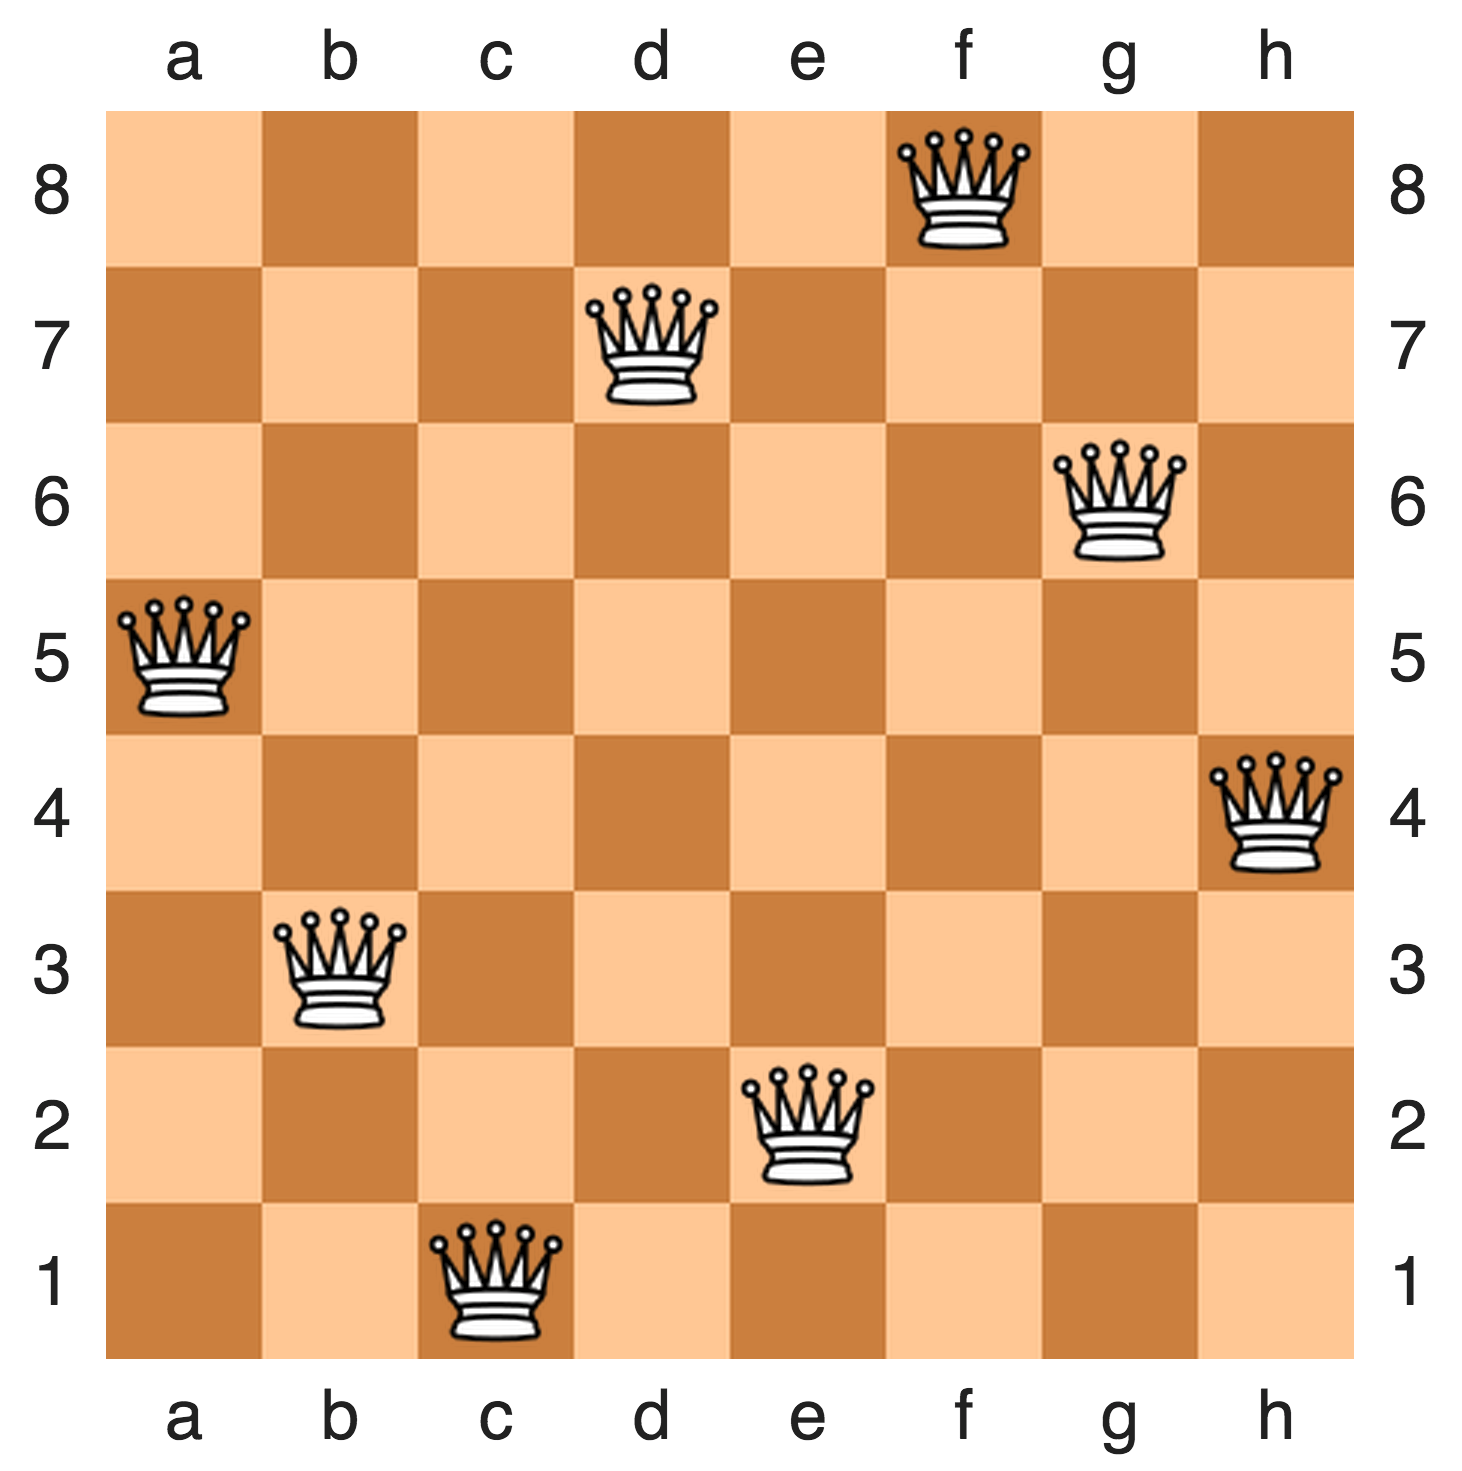
\includegraphics[width=0.5\textwidth]{nqueen-solution-8.png}
\end{figure}

Una solución válida es aquella donde no hay conflicto entre cualquier par de reinas en el tablero.
Por lo tanto, el valor de la función de aptitud será la cantidad de pares de reinas que no están en conflicto.
El valor máximo de la función de aptitud,
que usaremos como criterio de corte,
será $n \choose 2$.

\section{Herramientas de implementación}

Implementaremos una biblioteca propia en Scala.
El desarrollo actual puede verse en el siguiente repositorio: \url{https://github.com/rolodato/genetics}


\printbibliography

\end{document}